\documentclass{uimppracticas}

%Permitir cabeceras y pie de páginas personalizados
\pagestyle{fancy}

%Path por defecto de las imágenes
\graphicspath{ {./images/} }

%Declarar formato de encabezado y pie de página de las páginas del documento
\fancypagestyle{doc}{
  %Pie de Página
  \footerpr{}{}{{\thepage} de \pageref{LastPage}}
}

%Declarar formato de encabezado y pie del título e indice
\fancypagestyle{titu}{%
  %Cabecera
  \headerpr{}{}{}
  %Pie de Página
  \footerpr{}{}{}
}

\appto\frontmatter{\pagestyle{titu}}
\appto\mainmatter{\pagestyle{doc}}

\begin{document}
	
%Comienzo formato título
\frontmatter

%Portada (Centrado todo)
\centeredtitle{./images/LogoUIMP.png}{Máster Universitario en Investigación en Inteligencia Artificial}{Curso 2020-2021}{Recuperación y extracción de información, \\ grafos y redes sociales}{Análisis y Visualización Básica de una Red Social con Gephi}

\begin{center}
\large \today
\end{center}

\vspace{40mm}

\begin{flushright}
 	{\bf Laura Rodríguez Navas}\\
 	\textbf{DNI:} 43630508Z\\
 	\textbf{e-mail:} \href{rodrigueznavas@posgrado.uimp.es}{rodrigueznavas@posgrado.uimp.es}
\end{flushright}

\newpage

%Índice
% \tableofcontents

% \newpage

%Comienzo formato documento general
\mainmatter

\setlength\parskip{2.5ex}

\section*{La Red}

La red \textit{Diseasome}\cite{Goh8685} seleccionada para realizar esta práctica es una red de trastornos y genes de diferentes enfermedades vinculadas por asociaciones conocidas entre trastornos y genes, que nos indican el origen genético común de muchas enfermedades. La forman 526 enfermedades y 903 genes, donde los genes asociados con trastornos similares muestran una mayor probabilidad de interacciones físicas entre sus productos y una mayor similitud de perfiles de expresión para sus transcripciones, lo que respalda la existencia de distintos módulos funcionales específicos de la enfermedad. 

Se puede descargar en el siguiente enlace: \url{http://gephi.org/datasets/diseasome.gexf.zip} y una vez descargada, se descomprime el fichero que la contiene y se carga en \textit{Gephi}\cite{Gephi} para realizar las tareas básicas de análisis y visualización. 

La primera tarea es generar una imagen de la red completa y otra de la componente gigante. 

\begin{figure}[h]
	\centering
	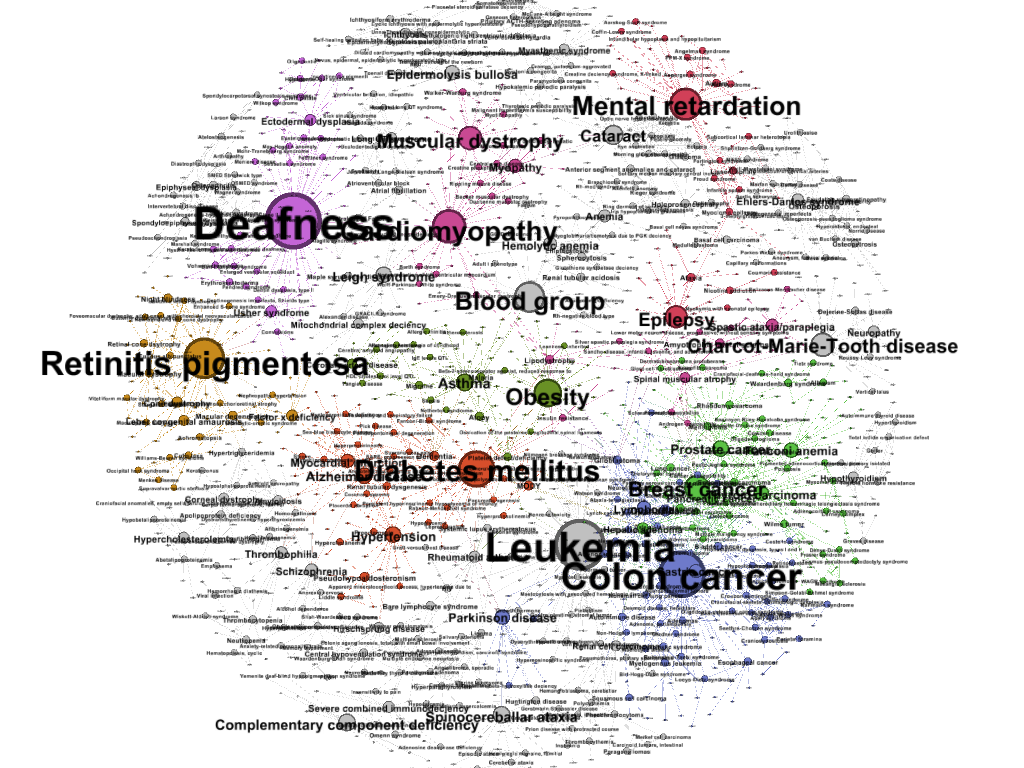
\includegraphics[width=0.9\textwidth]{images/completa_FR_labels}
	\caption{Imagen de la red completa con Fruchterman Reingold.}
\end{figure}

Las diferentes enfermedades están agrupadas por colores. Los nodos grises representan las enfermedades y los genes. Las aristas representan las correlaciones entre las enfermedades y los genes, o las relaciones entre enfermedades si tienen un gen en común. El tamaño de la etiqueta depende del tamaño del nodo. Está claro que los cánceres son la enfermedad más dominante de todas. La sordera también se lleva una gran porción.

\begin{figure}[h]
	\centering
	% \includegraphics[width=0.25\textwidth]{contour}
	\caption{Imagen de la componente gigante.}
\end{figure}

\section*{Análisis Básico de la Red}


\section*{Estudio de la Centralidad de los Actores}

\section*{Visualizaciones y Gráficos adicionales}

\newpage

\renewcommand{\refname}{Bibliografía}
\bibliographystyle{unsrt}
\bibliography{biblio}

\end{document}
